% ============================================================
% Question Bank: ch05-01 Writing Two-Step Equations from Word Problems
% Topic Title: Writing Two-Step Equations from Word Problems
% CCSS: 7.EE.B.4a
% Questions: 27 (15 MC + 6 SA + 6 Graphical)
% ============================================================

% --- Multiple Choice Questions (15) ---

\begin{practiceQuestion}{5-1-q01}{mc}
\begin{questionText}
A tutoring center charges $\$20$ per session plus a one-time registration fee of $\$35$. A student paid $\$155$ total. Which equation finds the number of sessions $s$?
\end{questionText}
\choiceA{$35s + 20 = 155$}
\choiceB{$20s + 35 = 155$}
\choiceC{$20s - 35 = 155$}
\choiceD{$55s = 155$}
\correctAnswer{B}
\explanation{Each session costs $\$20$, so $s$ sessions cost $20s$. Add the $\$35$ registration fee: $20s + 35 = 155$.}
\end{practiceQuestion}

\begin{practiceQuestion}{5-1-q02}{mc}
\begin{questionText}
``Six times a number, decreased by $11$, equals $43$.'' Which equation matches this statement?
\end{questionText}
\choiceA{$6(n - 11) = 43$}
\choiceB{$11 - 6n = 43$}
\choiceC{$6n - 11 = 43$}
\choiceD{$6n + 11 = 43$}
\correctAnswer{C}
\explanation{``Six times a number'' is $6n$. ``Decreased by $11$'' gives $6n - 11$. ``Equals $43$'' gives $6n - 11 = 43$.}
\end{practiceQuestion}

\begin{practiceQuestion}{5-1-q03}{mc}
\begin{questionText}
A water tank holds $350$ gallons and loses $15$ gallons per hour through a leak. After $h$ hours, $110$ gallons remain. Which equation models this situation?
\end{questionText}
\choiceA{$350 + 15h = 110$}
\choiceB{$15h - 350 = 110$}
\choiceC{$350 - 15h = 110$}
\choiceD{$110 + 350 = 15h$}
\correctAnswer{C}
\explanation{Start with $350$ gallons and lose $15$ per hour: $350 - 15h$. Set equal to the remaining $110$ gallons: $350 - 15h = 110$.}
\end{practiceQuestion}

\begin{practiceQuestion}{5-1-q04}{mc}
\begin{questionText}
A concert venue sells tickets for $\$t$ each. After selling $6$ tickets and receiving a $\$50$ donation, the venue collected $\$170$. Which equation finds the ticket price?
\end{questionText}
\choiceA{$6t - 50 = 170$}
\choiceB{$50t + 6 = 170$}
\choiceC{$6t + 50 = 170$}
\choiceD{$6 + 50t = 170$}
\correctAnswer{C}
\explanation{Six tickets at $\$t$ each is $6t$, plus the $\$50$ donation: $6t + 50 = 170$.}
\end{practiceQuestion}

\begin{practiceQuestion}{5-1-q05}{mc}
\begin{questionText}
``A number divided by $4$, plus $9$, equals $17$.'' Which equation matches?
\end{questionText}
\choiceA{$\dfrac{n + 9}{4} = 17$}
\choiceB{$\dfrac{n}{4} - 9 = 17$}
\choiceC{$4n + 9 = 17$}
\choiceD{$\dfrac{n}{4} + 9 = 17$}
\correctAnswer{D}
\explanation{``A number divided by $4$'' is $\frac{n}{4}$. ``Plus $9$'' gives $\frac{n}{4} + 9$. ``Equals $17$'' gives $\frac{n}{4} + 9 = 17$.}
\end{practiceQuestion}

\begin{practiceQuestion}{5-1-q06}{mc}
\begin{questionText}
A lawn-care service charges $\$40$ per yard plus a $\$25$ travel fee. The total bill was $\$185$. Which equation finds the number of yards $y$?
\end{questionText}
\choiceA{$25y + 40 = 185$}
\choiceB{$40y - 25 = 185$}
\choiceC{$65y = 185$}
\choiceD{$40y + 25 = 185$}
\correctAnswer{D}
\explanation{Each yard costs $\$40$, so $y$ yards cost $40y$. Add the $\$25$ travel fee: $40y + 25 = 185$.}
\end{practiceQuestion}

\begin{practiceQuestion}{5-1-q07}{mc}
\begin{questionText}
Which situation could be modeled by the equation $5x - 12 = 38$?
\end{questionText}
\choiceA{You buy $5$ items at $\$x$ each and use a $\$12$ coupon. You pay $\$38$.}
\choiceB{You earn $\$5$ per hour plus $\$12$ already saved. You have $\$38$.}
\choiceC{You split $\$38$ among $5$ people and each gets $\$12$.}
\choiceD{You save $\$12$ per week for $5$ weeks and have $\$38$.}
\correctAnswer{A}
\explanation{$5$ items at $\$x$ each is $5x$. Subtracting the $\$12$ coupon gives $5x - 12$. The total is $\$38$: $5x - 12 = 38$.}
\end{practiceQuestion}

\begin{practiceQuestion}{5-1-q08}{mc}
\begin{questionText}
``Eight more than three times a number is $-7$.'' Which equation matches?
\end{questionText}
\choiceA{$3n - 8 = -7$}
\choiceB{$8n + 3 = -7$}
\choiceC{$3(n + 8) = -7$}
\choiceD{$3n + 8 = -7$}
\correctAnswer{D}
\explanation{``Three times a number'' is $3n$. ``Eight more than'' means add $8$: $3n + 8$. ``Is $-7$'' gives $3n + 8 = -7$.}
\end{practiceQuestion}

\begin{practiceQuestion}{5-1-q09}{mc}
\begin{questionText}
A hiker has climbed $200$ feet and gains $30$ feet per minute. After $m$ minutes she is at $680$ feet. Which equation represents this?
\end{questionText}
\choiceA{$200m + 30 = 680$}
\choiceB{$30m - 200 = 680$}
\choiceC{$30m + 200 = 680$}
\choiceD{$680 - 30m = 200$}
\correctAnswer{C}
\explanation{Start at $200$ feet and gain $30$ per minute: $30m + 200 = 680$.}
\end{practiceQuestion}

\begin{practiceQuestion}{5-1-q10}{mc}
\begin{questionText}
A printer has $500$ sheets of paper. It uses $22$ sheets for each copy of a report. After printing $c$ copies, $r$ sheets remain. Which equation is correct?
\end{questionText}
\choiceA{$500 + 22c = r$}
\choiceB{$22c - 500 = r$}
\choiceC{$500 - 22c = r$}
\choiceD{$500c - 22 = r$}
\correctAnswer{C}
\explanation{Start with $500$ sheets and subtract $22$ per copy: $500 - 22c = r$.}
\end{practiceQuestion}

\begin{practiceQuestion}{5-1-q11}{mc}
\begin{questionText}
A streaming service charges $\$0.99$ per movie plus a $\$9.99$ monthly fee. Your bill was $\$16.95$. Which equation finds the number of movies $m$ you rented?
\end{questionText}
\choiceA{$9.99m + 0.99 = 16.95$}
\choiceB{$0.99m + 9.99 = 16.95$}
\choiceC{$0.99m - 9.99 = 16.95$}
\choiceD{$10.98m = 16.95$}
\correctAnswer{B}
\explanation{Each movie costs $\$0.99$, so $m$ movies cost $0.99m$. Add the $\$9.99$ fee: $0.99m + 9.99 = 16.95$.}
\end{practiceQuestion}

\begin{practiceQuestion}{5-1-q12}{mc}
\begin{questionText}
``Fifteen less than a number divided by $3$ is $2$.'' Which equation matches this statement?
\end{questionText}
\choiceA{$\dfrac{n}{3} + 15 = 2$}
\choiceB{$15 - \dfrac{n}{3} = 2$}
\choiceC{$\dfrac{n - 15}{3} = 2$}
\choiceD{$\dfrac{n}{3} - 15 = 2$}
\correctAnswer{D}
\explanation{``A number divided by $3$'' is $\frac{n}{3}$. ``Fifteen less than'' means subtract $15$: $\frac{n}{3} - 15$. ``Is $2$'' gives $\frac{n}{3} - 15 = 2$.}
\end{practiceQuestion}

\begin{practiceQuestion}{5-1-q13}{mc}
\begin{questionText}
A baker makes $d$ dozen cookies per batch. She makes $4$ batches and eats $6$ cookies. She has $186$ cookies left. Which equation finds $d$?
\end{questionText}
\choiceA{$4d - 6 = 186$}
\choiceB{$12 \times 4d - 6 = 186$}
\choiceC{$4(12d) - 6 = 186$}
\choiceD{$48d + 6 = 186$}
\correctAnswer{C}
\explanation{Each batch has $12d$ cookies. Four batches give $4(12d) = 48d$ cookies. After eating $6$: $48d - 6 = 186$. Choice C simplifies to the same equation.}
\end{practiceQuestion}

\begin{practiceQuestion}{5-1-q14}{mc}
\begin{questionText}
You owe your sister $\$75$. You pay her $\$11$ each week. After $w$ weeks you still owe $\$9$. Which equation models this?
\end{questionText}
\choiceA{$75 + 11w = 9$}
\choiceB{$11w - 75 = 9$}
\choiceC{$75 - 11w = 9$}
\choiceD{$75w - 11 = 9$}
\correctAnswer{C}
\explanation{Start owing $\$75$ and pay $\$11$ per week: $75 - 11w$. You still owe $\$9$: $75 - 11w = 9$.}
\end{practiceQuestion}

\begin{practiceQuestion}{5-1-q15}{mc}
\begin{questionText}
A florist sells bouquets for $\$18$ each. She also sells a vase for $\$12$. A customer buys $b$ bouquets and one vase for a total of $\$66$. Which equation finds $b$?
\end{questionText}
\choiceA{$12b + 18 = 66$}
\choiceB{$18b - 12 = 66$}
\choiceC{$18b + 12 = 66$}
\choiceD{$30b = 66$}
\correctAnswer{C}
\explanation{$b$ bouquets at $\$18$ each is $18b$. Add the $\$12$ vase: $18b + 12 = 66$.}
\end{practiceQuestion}

% --- Short Answer Questions (6) ---

\begin{practiceQuestion}{5-1-q16}{sa}
\begin{questionText}
Write an equation: ``You buy $n$ T-shirts at $\$14$ each and pay $\$6$ for tax. The total is $\$76$.''
\end{questionText}
\correctAnswer{$14n + 6 = 76$}
\explanation{$n$ shirts at $\$14$ each is $14n$. Add $\$6$ tax: $14n + 6$. Set equal to $\$76$: $14n + 6 = 76$.}
\end{practiceQuestion}

\begin{practiceQuestion}{5-1-q17}{sa}
\begin{questionText}
A pool is being filled at a rate of $45$ gallons per minute. It already has $120$ gallons. Write an equation to find how many minutes $m$ until the pool has $1{,}470$ gallons.
\end{questionText}
\correctAnswer{$45m + 120 = 1{,}470$}
\explanation{Each minute adds $45$ gallons: $45m$. Plus the $120$ already present: $45m + 120 = 1{,}470$.}
\end{practiceQuestion}

\begin{practiceQuestion}{5-1-q18}{sa}
\begin{questionText}
Write an equation for: ``Four times a number, increased by $7$, is $-5$.''
\end{questionText}
\correctAnswer{$4n + 7 = -5$}
\explanation{``Four times a number'' is $4n$. ``Increased by $7$'' gives $4n + 7$. ``Is $-5$'' gives $4n + 7 = -5$.}
\end{practiceQuestion}

\begin{practiceQuestion}{5-1-q19}{sa}
\begin{questionText}
A dance studio charges $\$55$ per month plus $\$30$ per private lesson. A dancer's monthly bill was $\$205$. Write an equation to find the number of private lessons $p$.
\end{questionText}
\correctAnswer{$30p + 55 = 205$}
\explanation{$p$ private lessons cost $30p$. Add the $\$55$ monthly fee: $30p + 55 = 205$.}
\end{practiceQuestion}

\begin{practiceQuestion}{5-1-q20}{sa}
\begin{questionText}
A gift card has $\$100$. You spend $\$d$ per day. After $7$ days you have $\$23$ left. Write an equation.
\end{questionText}
\correctAnswer{$100 - 7d = 23$}
\explanation{Start with $\$100$ and subtract $\$d$ each day for $7$ days: $100 - 7d = 23$.}
\end{practiceQuestion}

\begin{practiceQuestion}{5-1-q21}{sa}
\begin{questionText}
Write an equation for: ``A number $n$ multiplied by $\dfrac{2}{3}$, then increased by $5$, equals $11$.''
\end{questionText}
\correctAnswer{$\dfrac{2}{3}n + 5 = 11$}
\explanation{``A number multiplied by $\frac{2}{3}$'' is $\frac{2}{3}n$. ``Increased by $5$'' gives $\frac{2}{3}n + 5$. ``Equals $11$'' gives $\frac{2}{3}n + 5 = 11$.}
\end{practiceQuestion}

% --- Graphical MC Questions (3) ---

\begin{practiceQuestion}{5-1-q22}{gmc}
\begin{questionText}
The diagram below shows a balance scale in equilibrium. Which equation represents the balance?

\begin{center}
\begin{tikzpicture}[scale=0.8]
  % Fulcrum
  \draw[thick] (0,-0.5) -- (-0.4,-1.2) -- (0.4,-1.2) -- cycle;
  % Beam
  \draw[thick] (-4,0) -- (4,0);
  % Left pan
  \draw[thick] (-4,0) -- (-4.5,-0.5) -- (-3.5,-0.5) -- (-4,0);
  \draw[thick,fill=funBlue!20] (-4.5,-0.5) -- (-4.5,-0.8) -- (-3.5,-0.8) -- (-3.5,-0.5) -- cycle;
  \node at (-4,-0.65) {\small $5x + 8$};
  % Right pan
  \draw[thick] (4,0) -- (4.5,-0.5) -- (3.5,-0.5) -- (4,0);
  \draw[thick,fill=funOrange!20] (4.5,-0.5) -- (4.5,-0.8) -- (3.5,-0.8) -- (3.5,-0.5) -- cycle;
  \node at (4,-0.65) {\small $63$};
\end{tikzpicture}
\end{center}
\end{questionText}
\choiceA{$5x - 8 = 63$}
\choiceB{$8x + 5 = 63$}
\choiceC{$5x + 8 = 63$}
\choiceD{$5 + 8x = 63$}
\correctAnswer{C}
\explanation{The left pan shows $5x + 8$ and the right pan shows $63$. Since the scale is balanced, $5x + 8 = 63$.}
\end{practiceQuestion}

\begin{practiceQuestion}{5-1-q23}{gmc}
\begin{questionText}
The table shows the relationship between hours worked and total earnings. Which equation models the data?

\begin{center}
\begin{tabular}{|c|c|}
\hline
\textbf{Hours ($h$)} & \textbf{Earnings (\$)} \\
\hline
$1$ & $\$22$ \\
\hline
$2$ & $\$34$ \\
\hline
$3$ & $\$46$ \\
\hline
$4$ & $\$58$ \\
\hline
\end{tabular}
\end{center}
\end{questionText}
\choiceA{$12h + 10 = E$}
\choiceB{$22h = E$}
\choiceC{$10h + 12 = E$}
\choiceD{$12h + 22 = E$}
\correctAnswer{A}
\explanation{The earnings increase by $\$12$ per hour (rate), so the hourly rate is $12$. When $h = 1$: $12(1) + 10 = 22$ \checkmark. The equation is $12h + 10 = E$.}
\end{practiceQuestion}

\begin{practiceQuestion}{5-1-q24}{gmc}
\begin{questionText}
The diagram shows a rectangle with a perimeter of $58$ cm. Which equation can be used to find $x$?

\begin{center}
\begin{tikzpicture}[scale=0.6]
  \draw[thick,fill=funBlue!10] (0,0) rectangle (8,3);
  \draw[<->] (0,-0.5) -- (8,-0.5);
  \node[below] at (4,-0.5) {$x + 7$ cm};
  \draw[<->] (8.5,0) -- (8.5,3);
  \node[right] at (8.5,1.5) {$x$ cm};
\end{tikzpicture}
\end{center}
\end{questionText}
\choiceA{$2x + 7 = 58$}
\choiceB{$4x + 14 = 58$}
\choiceC{$x(x + 7) = 58$}
\choiceD{$2x + 14 = 58$}
\correctAnswer{B}
\explanation{Perimeter $= 2(x + 7) + 2x = 2x + 14 + 2x = 4x + 14$. Set equal to $58$: $4x + 14 = 58$.}
\end{practiceQuestion}

% --- Graphical SA Questions (3) ---

\begin{practiceQuestion}{5-1-q25}{gsa}
\begin{questionText}
The balance scale below is in equilibrium. Write an equation that represents the balance.

\begin{center}
\begin{tikzpicture}[scale=0.8]
  % Fulcrum
  \draw[thick] (0,-0.5) -- (-0.4,-1.2) -- (0.4,-1.2) -- cycle;
  % Beam
  \draw[thick] (-4,0) -- (4,0);
  % Left pan
  \draw[thick] (-4,0) -- (-4.5,-0.5) -- (-3.5,-0.5) -- (-4,0);
  \draw[thick,fill=funBlue!20] (-4.5,-0.5) -- (-4.5,-0.8) -- (-3.5,-0.8) -- (-3.5,-0.5) -- cycle;
  % Left: 3 boxes labeled n + one block labeled 15
  \node[draw,fill=funBlue!40,minimum size=0.35cm] at (-4.3,-1.2) {\small $n$};
  \node[draw,fill=funBlue!40,minimum size=0.35cm] at (-4.0,-1.2) {\small $n$};
  \node[draw,fill=funBlue!40,minimum size=0.35cm] at (-3.7,-1.2) {\small $n$};
  \node[draw,fill=funOrange!40,minimum size=0.35cm] at (-4.0,-1.6) {\small $15$};
  % Right pan
  \draw[thick] (4,0) -- (4.5,-0.5) -- (3.5,-0.5) -- (4,0);
  \draw[thick,fill=funOrange!20] (4.5,-0.5) -- (4.5,-0.8) -- (3.5,-0.8) -- (3.5,-0.5) -- cycle;
  \node at (4,-0.65) {\small $72$};
\end{tikzpicture}
\end{center}
\end{questionText}
\correctAnswer{$3n + 15 = 72$}
\explanation{The left pan has $3$ boxes of $n$ and one block of $15$, giving $3n + 15$. The right pan has $72$. Since the scale balances, $3n + 15 = 72$.}
\end{practiceQuestion}

\begin{practiceQuestion}{5-1-q26}{gsa}
\begin{questionText}
The table shows the cost for different numbers of ride tickets at a carnival, including a $\$5$ entry fee. Write an equation for the total cost $C$ in terms of the number of tickets $t$.

\begin{center}
\begin{tabular}{|c|c|}
\hline
\textbf{Tickets ($t$)} & \textbf{Total Cost ($C$)} \\
\hline
$0$ & $\$5$ \\
\hline
$3$ & $\$11$ \\
\hline
$6$ & $\$17$ \\
\hline
$9$ & $\$23$ \\
\hline
\end{tabular}
\end{center}
\end{questionText}
\correctAnswer{$C = 2t + 5$}
\explanation{The entry fee is $\$5$ (the cost when $t = 0$). Each $3$ additional tickets add $\$6$, so each ticket costs $\$2$. The equation is $C = 2t + 5$.}
\end{practiceQuestion}

\begin{practiceQuestion}{5-1-q27}{gsa}
\begin{questionText}
A garden has the shape shown below. Write an equation to find $x$ if the total perimeter is $88$ feet.

\begin{center}
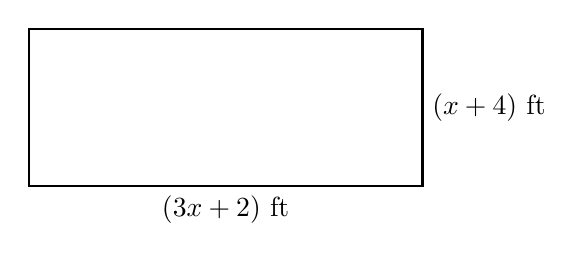
\begin{tikzpicture}[scale=0.5]
  \draw[thick] (0,0) -- (10,0) -- (10,4) -- (0,4) -- cycle;
  \node[below] at (5,0) {$(3x + 2)$ ft};
  \node[right] at (10,2) {$(x + 4)$ ft};
\end{tikzpicture}
\end{center}
\end{questionText}
\correctAnswer{$2(3x + 2) + 2(x + 4) = 88$}
\explanation{The perimeter of a rectangle is $2 \times \text{length} + 2 \times \text{width}$: $2(3x + 2) + 2(x + 4) = 88$, which simplifies to $8x + 12 = 88$.}
\end{practiceQuestion}
